\newcommand{\dotted}[0]{\makedash{2pt}}
\newcommand{\g}[1]{{\footnotesize $#1$}}

\section{TAG}

\outline{

\begin{itemize}
\item Begriffe
\item Phrasenstrukturgrammatiken
\item Government \& Binding (GB)
\item Generalisierte Phrasenstrukturgrammatik (GPSG)
\item Lexikalisch-Funktionale Grammatik (LFG)
%\item Lexical Mapping Theory (LMT)
%\item PATR
\item Kategorialgrammatik (CG)
\item Kopfgesteuerte Phrasenstrukturgrammatik (HPSG)
\item Konstruktionsgrammatik (CxG)
\item \blau{Baumadjunktionsgrammatik (TAG)}
\end{itemize}
}


\frame{
\frametitle{Tree Adjoining Grammar (TAG)}


\begin{itemize}[<+->]
\item \emph{Tree Adjoining Grammar} (TAG) wurde von Aravind Joshi entwickelt.
\item TAG ist interessant, weil man annimmt,\\
  daß dieser Grammatikformalismus von seiner
  Ausdrucksmächtigkeit ziemlich genau das kann, was Menschen auch können, wenn sie natürliche
  Sprache produzieren oder rezipieren.
\item wichtige Aufsätze:\\
      \citew*{JLT75a-u,Joshi87a-u,JS97a} \\
Zum Deutschen: \citew*{JBR2000a}
% sind die Aufsätze von Owen Rambow wichtig

\end{itemize}

}

\subsection{Allgemeines zum Repräsentationsformat}

\frame{
\frametitle{Allgemeines zum Repräsentationsformat}

\begin{itemize}
\item Die Grundidee ist einfach: Man ordnet jedem Kopf einen Baum zu,\\
     der eine Struktur beschreibt, in der der Kopf vorkommen kann. 

\pause
\item Solche Bäume können mit zwei Operationen zu komplexeren Bäumen zusammengebaut werden: Substitution
und Adjunktion.
\end{itemize}


}

\subsubsection{Elementare Bäume ({\em Elementary Trees})}

\frame{
\frametitle{Elementare Bäume (\emph{Elementary Trees})}

\vfill


\hfill
\begin{forest}
tag
[NP
	[John]]
\end{forest}
\hfill
\begin{forest}
tag
[S
	[NP$\downarrow$]
	[VP
		[V
			[laughs]]]]
\end{forest}
\hfill
\begin{forest}
tag
[VP
	[ADV
		[always]]
	[VP*]]
\end{forest}
\hfill\mbox{}

\vfill

Knoten für Einsetzungen von Argumenten sind speziell markiert\\
(NP im Baum für \emph{laughs}).

Knoten für Einsetzungen von Adjunkten in einen Baum sind ebenfalls markiert (VP im Baum für \emph{always}).

\vfill
}

\subsubsection{Substitution}

\frame{
\frametitle{Substitution}

\vfill
\centerline{%
\begin{forest}
tag
[S
	[NP$\downarrow$,
          [NP, substitution
            [John]]]
	[VP
		[V
			[laughs]]]]
\end{forest}
\hspace{1em}
\raisebox{1cm}{$\leadsto$}
\hspace{1em}
\begin{forest}
tag
[S
	[NP
		[John]]
	[VP
		[V
			[laughs]]]]
\end{forest}
}

\vfill
An Substitutionsknoten müssen andere Teilbäume eingesetzt werden.

\vfill

}

\subsubsection{Adjunktion}


\frame{
\frametitle{Adjunktion}

\vfill
\centerline{%
\begin{forest}
tag
[S
	[NP
		[John]]
	[VP
		[V
			[laughs]]]]
\end{forest}
\hspace{0.5cm}
\begin{forest}
tag
[VP
	[ADV
		[always]]
	[VP*]]
\end{forest}
\hspace{1em}
\raisebox{1cm}{$\leadsto$}
\hspace{1em}
\begin{forest}
tag
[S
	[NP
		[John]]
	[VP
		[ADV
			[always]]
		[VP
			[V
				[laughs]]]]]
\end{forest}
}

\vfill
Adjunktionsbäume können in einen anderen Baum eingefügt werden.
\vfill

}


\subsection{Lokale Umstellungen}

\frame{
\frametitle{Lokale Umstellungen}


\begin{itemize}[<+->]
\item Zu jedem Wort gibt es eine Familie von Bäumen.
\item Zu einem ditransitivem Verb gibt es unter anderem sechs Bäume,\\
die den verschiedenen  Anordnungen der Argumente entsprechen.
\item Die Bäume werden über Lexikonregeln in Beziehung zueinander gesetzt.
\item TAG kann Umordnungen nicht behandeln,\\
      wenn Argumente verschiedener Verben abwechselnd auftreten.
\item Für solche Fälle braucht man eine Erweiterung des TAG-Formalismus: Multi-Component TAG.\\
      Zu den Details siehe \citew*{JBR2000a}.
\end{itemize}



}

\subsection{Passiv}

\frame{
\frametitle{Passiv}


\begin{itemize}[<+->]
\item Zu jedem Wort gibt es eine Familie von Bäumen.
\item Zu einem Aktiv"=Baum gehört ein Passiv-Baum.
\item Diese werden über Lexikonregeln in Beziehung zueinander gesetzt.
\item Die Lexikonregeln entsprechen den Transformationen der \gbt,\\
      die Bäume auf Bäume abbilden.
\end{itemize}


}

\subsection{Fernabhängigkeiten}


\frame{
\frametitle{Fernabhängigkeiten}

\vfill
Es werden einfach Bäume in die Mitte anderer Bäume eingesetzt.
\vfill


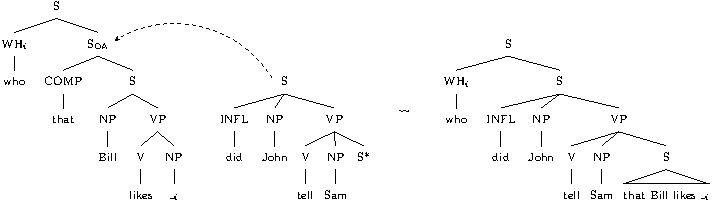
\includegraphics[width=\textwidth]{Figures/tag-long-distance-dependencies-crop}

%% \oneline{%
%% \begin{forest}
%% tag
%% [S
%% 	[WH$_i$
%% 		[who]]
%% 	[%\tikzmark{soa}{S\sub{OA}}
%%          S\sub{OA},name=soa
%% 		[COMP
%% 			[that]]
%% 		[S
%% 			[NP
%% 				[Bill]]
%% 			[VP
%% 				[V
%% 					[likes]]
%% 				[NP
%% 					[\noexpand\_$_i$]]]]]]
%% \end{forest}
%% %}
%% %\hspace{0.5cm}
%% \qquad
%% %\scalebox{.5}{%
%% \begin{forest}
%% tag
%% [S,name=s%\tikzmark{s}{S}
%% 	[INFL
%% 		[did]]
%% 	[NP
%% 		[John]]
%% 	[VP
%% 		[V
%% 			[tell]]
%% 		[NP
%% 			[Sam]]
%% 		[S*]]]
%% \end{forest}
%% %}
%% \qquad \raisebox{2cm}{$\rightsquigarrow$} \qquad
%% %\scalebox{.5}{%
%% \begin{forest}
%% tag
%% [S
%% 	[WH$_i$
%% 		[who]]
%% 	[S
%% 		[INFL
%% 			[did]]
%% 		[NP
%% 			[John]]
%% 		[VP
%% 			[V
%% 				[tell]]
%% 			[NP
%% 				[Sam]]
%% 			[S
%% 				[that Bill likes \noexpand\_$_i$, roof]]]]]
%% \end{forest}
%% \begin{tikzpicture}[overlay,remember picture]
%% \draw[->, dashed, bend angle=45, bend right] ($(pic cs:s)+(-0.25,0.2)$) to($(pic cs:soa)+(0.8,.2)$);
%% \end{tikzpicture}
%% }

\vfill

\eal
\ex \blaubf{who$_i$} did John tell Sam \blaubf{that Bill likes \_$_i$}\\
\pause
\ex \blaubf{who$_i$} did John tell Sam that Mary said \blaubf{that Bill likes \_$_i$}
\zl

\vfill



}

\frame{
\frametitle{Noch einige Details}

\begin{itemize}
\item Der Baum für \emph{WH COMP NP likes \_$_i$} gehört zur Baumfamilie von \emph{likes} und steht
  somit im Lexikon.
\item Obwohl der Baum für (\mex{1}) die Kategorie S hat, ist (\mex{1})  kein grammatischer
  Satz des Englischen.
\ea[*]{
who that Bill likes
}
\z
\pause
Die Markierung OA sagt, daß an der entsprechenden Stelle eine obligatorische Adjunktion stattfinden
muß.

\end{itemize}


}


\frame{
\frametitle{Idiome in TAG}

Idiom-Analyse ganz einfach. \citet{AS89a}:

\centerline{
\scalebox{.9}{%
\begin{forest}
tag
[S
	[NP$\downarrow$]
	[VP
		[V
			[takes]]
		[NP$\downarrow$]
		[PP$_{{\mathrm{NA}}}$
			[P
				[into]]
			[NP$_{\mathrm{NA}}$
				[N$_{\mathrm{NA}}$
					[account]]]]]]
\end{forest}
}}

}


